The game being challenging largely has to do with items 2, 5 and 6 of the requirements in section \ref{gamedesign:selectionofgametype:importantstuff}.
The challenge in the game is the horde of enemies that chase the player, but if the enemies are all stuck behind a wall the challenge is non-existent.
Therefore the enemies need to be able to avoid obstacles and chase the players in a intelligent way.
This could be achieved by applying a pathfinding algorithm to the AI's behaviour.
The process of creating an adequate pathfinding algorithm for our game was a three iteration process involving different optimizations to the algorithm.

\section{First Iteration}
Our initial idea was to simply create a tile graph\cite{AIG:Millington} as illustrated in \ref{gridGraph}.
A node would then have up to eight connections which would point to a neighbour of that certain node with a cost of traversing to this node.
Possible neighbours would be four to each side of the node with a cost of 10 and four diagonal neighbours with a cost of 14, which is the length of the hypotenuse when the length of the catheti are 10.

To navigate in the graph a pathfinding algorithm is needed. 
The pathfinding algorithm that would be used is the A* search pathfinding which has a runtime of $O(n \times m)$, where $n$ is the number of nodes that will be explored, $m$ is the average number of neighbours in the graph, and it is assumed that the graph and heuristic operations take constant time\cite{AIG:Millington}.

\begin{figure}[h]
	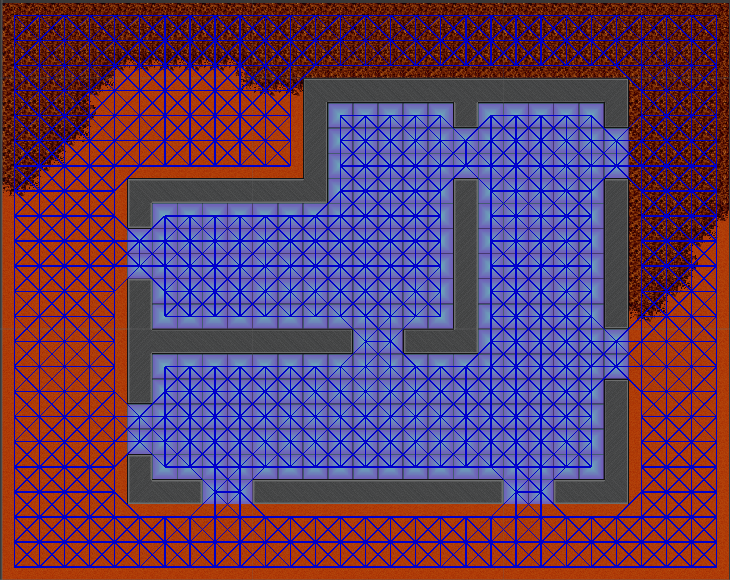
\includegraphics[width=\textwidth]{figures/astar/gridGraph}
	\caption{Graph based on the tiles of the map}
	\label{gridGraph}
\end{figure}

\subsection*{Choosing a heuristic}
The heuristic should be easily calculated and somewhat precise since it is to be called on runtime.
It is desired to have a heuristic which underestimates since overestimating can result in an incorrect shortest-path.
When working with tile maps three different heuristics are commonly used\cite{heuristics}:
\begin{itemize}
\item Manhattan Distance
\item Chebyshev Distance
\item Euclidean Distance
\end{itemize}
The Manhattan distance works very well on tile based maps. 
It is a simple heuristic, it works by adding the distance between the current node's x-coordinate and the goal node's x-coordinate, and the distance between the current node's y-coordinate and the goal node's y-coordinate.
However, it does not support diagonal movement. 
This means the heuristic will have a tendency to overestimate which will make it non-admissible heuristic.\\\\
The Chebyshev distance works almost in the same way, however, this heuristic take diagonal movement into account. 
It assumes that diagonal cost is equal to the side costs, this results in an underestimation or an exact cost of the path.\\\\
The last heuristic uses the euclidean distance between the current node and the goal node as the heuristic.
This however is more expensive to calculate.\\\\
Looking at these heuristics we find that the best prospect for our heuristic will be Chebyshev since it is faster than euclidean. 
Furthermore, it does not overestimate when dealing with diagonal movement as Manhatten does.

\subsection*{Checking for players in line of sight}
Upon seeing a player the enemies should begin to run after the players in a straight line and neglect their pathfinding. 
This would be done with Unity's raycasting system which would send out a ``ray'' in the direction of the player. 
If this ray would hit a wall the enemy would keep using A* to navigate after the player.
However, if the ray would hit a player the enemy will start hunting the player as illustrated in Figure \ref{raycast}.

This check is done continuous to ensure that if a player runs behind a wall the enemy would follow A* again to get to the player.
\begin{figure}[H]
\begin{center}
	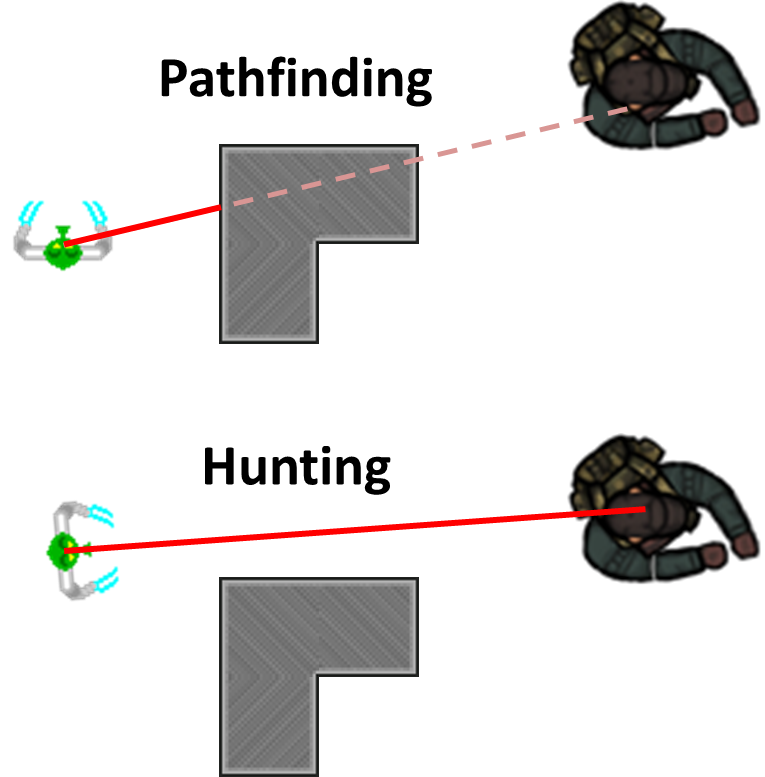
\includegraphics[width=0.5\textwidth]{figures/astar/raycast}
	\caption{Illustration of raycasting from a enemy to the character. Character Art by rileygombart\cite{artist}}
	\label{raycast}
\end{center}
\end{figure}

\subsection*{Result}
This approach resulted in a very large graph, an example would be a map of size 64x64, the graph created for that map has 3984 nodes and 30450 edges. Due to the size of the graph it will take a lot of time traverse through on runtime.
Furthermore we found the constant raycasting for each enemy was very expensive in terms of CPU usage, and had to be optimized.

\section{Second Iteration}
For the second iteration both the pathfinding and the raycasting had to be optimized since they both used to much of the CPU.

\subsection*{Optimizing pathfinding}
A way to optimize runtime performance of the pathfinding is to reduce the graph.
This would be done by creating a waypoint graph instead of a grid graph.
The waypoints would be created at the outer corners of the obstacles on the map, where the AI could make a turn, as seen in figure \ref{waypointsNode}.
Each point would then do a raycast to every other point to see if it was in direct line of sight, and if that was the case it was added as a neighbour and the cost of that edge would be the euclidean distance to that point.
A resulting graph can be seen in Figure \ref{waypointgraph}.
In comparison the old graph created had 3984 nodes and 30450 edges while this approach resulted in a much smaller graph with 47 nodes and 624 edges, thus improving both the creation and traversal times of the graph.

\begin{figure}[H]
\centering
\begin{minipage}{.5\textwidth}
\centering
	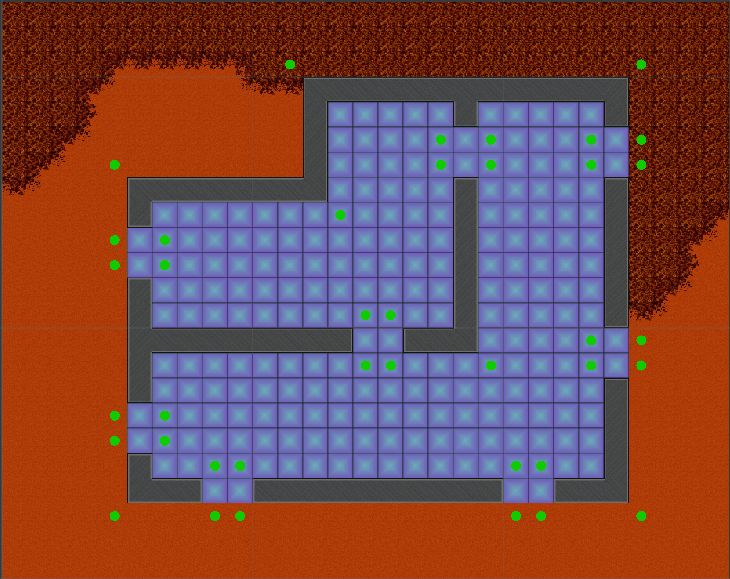
\includegraphics[width=0.9\textwidth]{figures/astar/waypoints}
	\caption{The placement of the waypoints}
	\label{waypointsNode}
	\end{minipage}%
\begin{minipage}{.5\textwidth}
\centering
	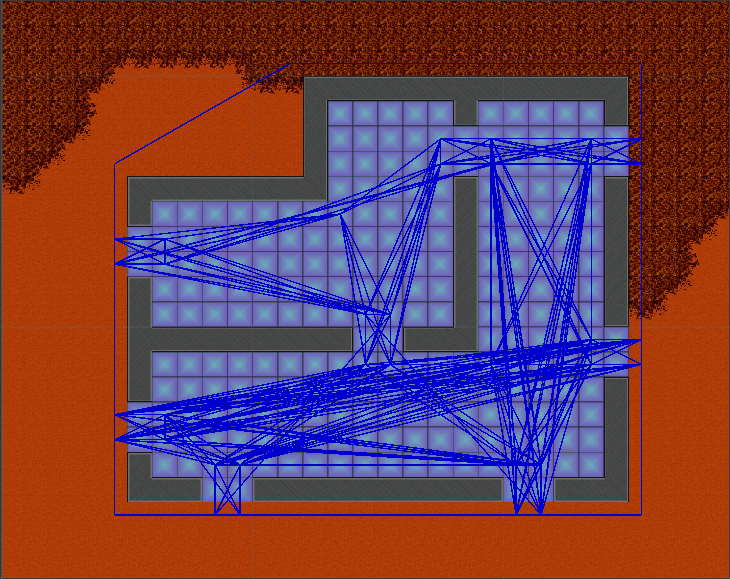
\includegraphics[width=0.9\textwidth]{figures/astar/waypointsGraph}
	\caption{Graph based on the waypoints}
	\label{waypointgraph}
	\end{minipage}
\end{figure}

This however raised a new problem, since there were fewer waypoints available the enemies had to find the nearest accessible waypoint.
To solve this the distances was calculated to each waypoint from the given position and then a ray was cast from the position of the enemy to the position of the nearest waypoint.
If the raycast hit an object the algorithm would move onto the second closest and so forth, as illustrated in Figure \ref{nearestWaypoint}.
\begin{figure}[H]
\begin{center}

	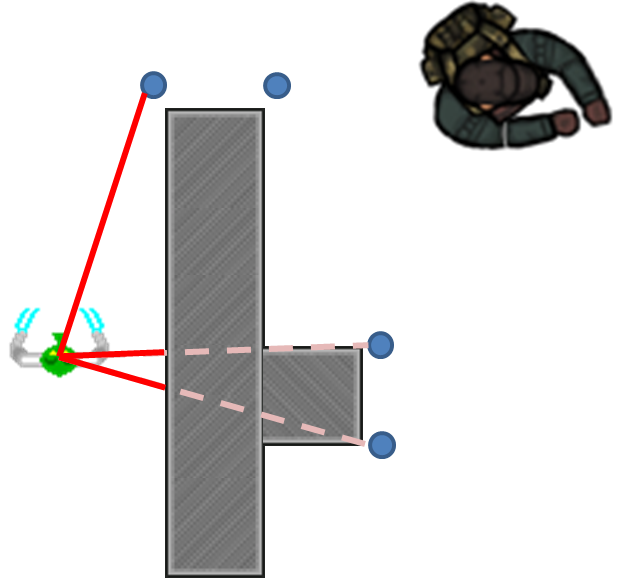
\includegraphics[width=0.4\textwidth]{figures/astar/findNearestWaypoint}
	\caption{Raycasts finding the nearest accessible waypoint. Character Art by rileygombart\cite{artist}}
	\label{nearestWaypoint}
	
\end{center}
\end{figure}

\subsection*{Minimizing of raycasting}
The minimizing of the raycasts is simply solved by adding a larger interval between each raycast.

\subsection*{Result}
While this solution had a much better performance, we found that the raycasting was still too CPU intensive and that it was desirable to remove it completely on runtime.
\section{Third Iteration}
For the third iteration was the goal to remove the raycasting that happens on runtime and to add other potential performance improvements.

\subsection*{Minimizing the Graph size}
It was possible to reduce the number of waypoints even further.
In order to do so all waypoints are looped through to find adjacent waypoints, meaning waypoints whose distance to each other is less or equal to one.
Those that are adjacent are then removed and a new waypoint is placed halfway between them.
This is illustrated in Figure \ref{waypointMerge}.
The resulting waypoints can be seen in Figure \ref{waypointOpt} with the graph in Figure \ref{waypointgraphOpt}. 
This can be compared to the old waypoint figure and graph shown in Figure \ref{waypointsNode} and Figure \ref{waypointgraph}.
Most notably, the amount of edges are significantly reduced.
\begin{figure}[H]
\begin{center}
	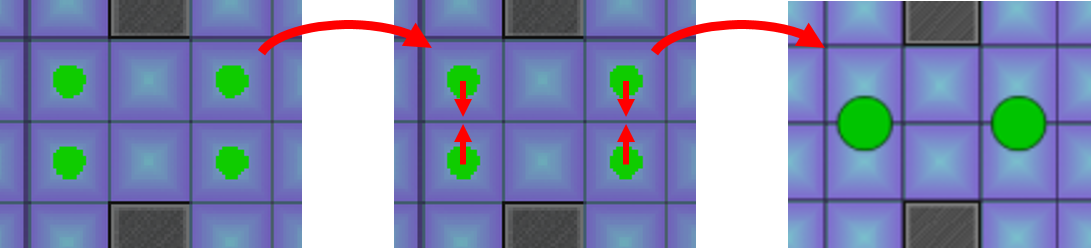
\includegraphics[width=\textwidth]{figures/astar/waypointMerge}
	\caption{Waypoint merging.}
	\label{waypointMerge}
\end{center}
\end{figure}

\begin{figure}[H]
\centering
	\begin{minipage}{.5\textwidth}
		\centering
		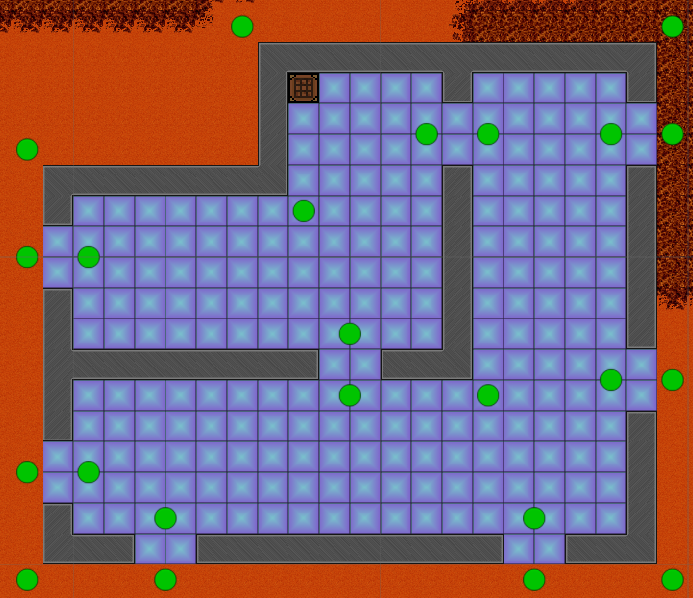
\includegraphics[scale=0.3]{figures/astar/optimizedWaypoints}
		\captionof{figure}{Waypoints after merge optimizations.}
		\label{waypointOpt}
	\end{minipage}%
	\begin{minipage}{.5\textwidth}
		\centering
		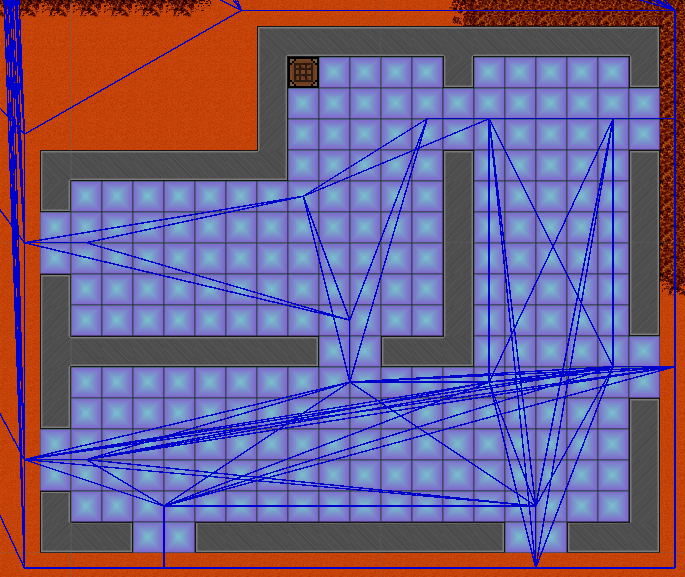
\includegraphics[scale=0.4]{figures/astar/optimizedWaypointsGraph}
		\captionof{figure}{Graph based on the waypoints after waypoint optimization.}
		\label{waypointgraphOpt}
	\end{minipage}
\end{figure}

\subsection*{Eliminating raycasts}
Raycast, in this case, is used to test if there is a straight, unobstructed path between two points in the game world.
This happens in two places:
\begin{itemize}
\item Between the positions of enemies and players
\item Between the positions of enemies and waypoints
\end{itemize}
The raycast from an enemy to a player happens when the enemy want to check if the enemy can ``see'' the player, i.e. the path to the player is unobstructed.
To prevent the raycast checks to the players, the map is partitioned into convex rectangles.
When an enemy then enters the same partition as a player it knows that it can walk directly towards the player since the rectangle is convex.
Such partitions are generated while also generating the backdrop.
For finding the rectangles to use for partitions, an inverted version of the algorithm used to walls, is used to find areas that are non-walls.
The resulting partitions of running the algorithm is illustrated in Figure~\ref{fig:partition_colliders_on_map}.

\begin{figure}[H]
\begin{center}
        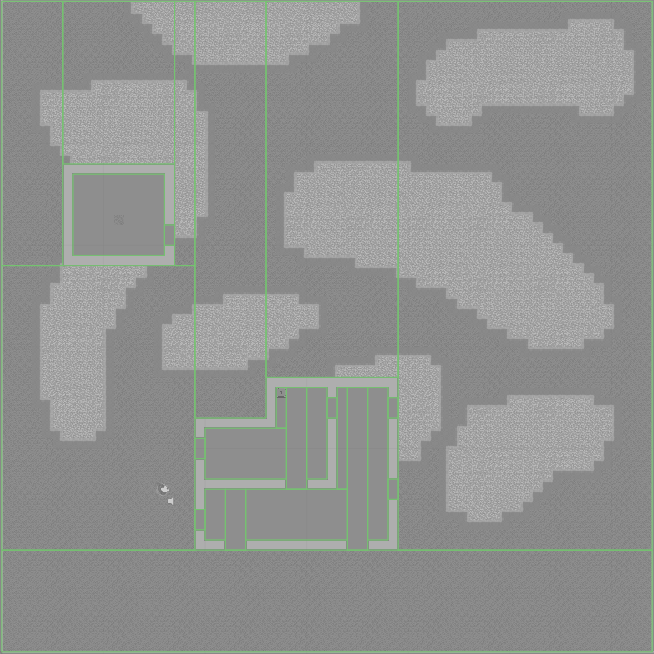
\includegraphics[width=0.9\textwidth]{figures/generating_levels/partition_colliders.png}
    \caption{Rectangles for partitions, separated by green lines.}\label{fig:partition_colliders_on_map}
\end{center}
\end{figure}

Once the partitions are made, trigger colliders are added to them.
Once a player or enemy collides with a partition, they will add a reference to that partition to their list of partitions.
Once they stop colliding with the partition they will remove it from their list of partitions.

\subsubsection*{Use of Partitions}
The enemy starts by checking whether it and the player are in the same partition and if so the enemy can go straight towards the player and the enemy will be in hunting mode.
In hunting mode, the enemy can also check neighbouring partitions for the player, such that if the player runs out of the partition, the enemy will still go straight towards the player.
This prevents odd behaviour from the enemies when they chase a players, since if there was no hunting mode the enemy would have to start pathfinding if the player leaves the partition, as illustrated in Figure \ref{huntingMode}.

\begin{figure}[H]
\begin{center}
        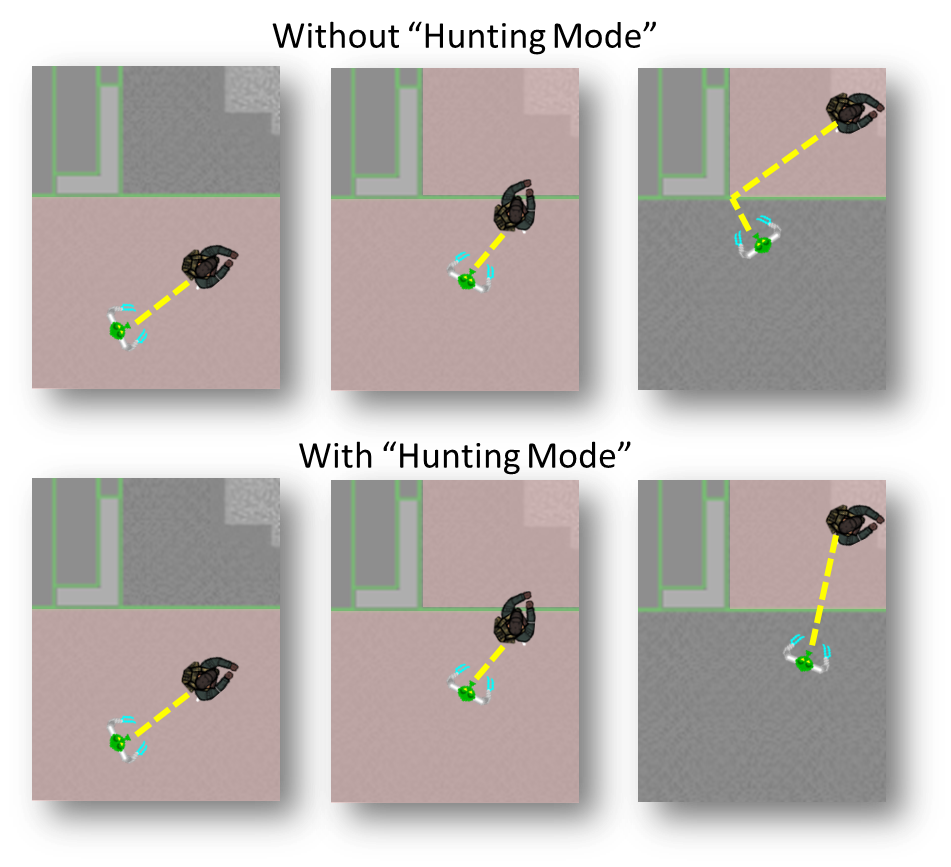
\includegraphics[width=\textwidth]{figures/astar/huntingMode.png}
    \caption{Behaviour difference between hunting mode and no hunting mode, showing if the players leave a partition the enemy without hunting mode would have to start pathfinding resulting in odd behaviour.}\label{huntingMode}
\end{center}
\end{figure}

If the player then escapes, meaning that the player is not in the same nor a neighbouring partitions, the enemy will start to run the pathfinding algorithm and follow the path.
The enemy will then run pathfinding again in $X$ seconds, where $X = \text{number of nodes in the path}$.
This is to recalculate the path in case the player has moved elsewhere since last run.
It is based on the number of nodes because that means enemies that aren't close to the player (and thus out of sight) will not take up as many resources.
The pathfinding continues until the enemy is in the same partition as the player again.

Running A* continuously while having a 50 enemies or more was still costly.
Therefore, the A* was moved to load time where it finds the shortest path for all the possible paths, and saves it in a hashtable.
That way, the pathfinding used during runtime is only lookups in the hashtable.
This is possible due to our relative low number of nodes and edges.\\
The last optimization was to eliminate the costly raycast happening when finding the nearest waypoints. 
This is done by adding the waypoints from the partition of the enemy and its neighbouring partitions into a list, then finding the one with the shortest distance. 
This ensures the closest accessible waypoint is found.

\subsection*{Result}
The result of this iteration was that all raycasting was removed from runtime and some of these raycasts were moved to load-time instead.
Furthermore A* calculations were moved to load-time which together with the waypoint-merge-optimization made the pathfinding algorithm work very effective, allowing us to reach a greater number of active enemies.

The trade-off from this improved performance is present if the player can move too quickly through partitions with a low number of waypoints.
As illustrated in Figure \ref{tradeoff}, the enemy can only hunt through two partitions, which leads to the enemy having odd looking behaviour if the player runs too quickly through the partitions.
\begin{figure}[H]
\begin{center}
        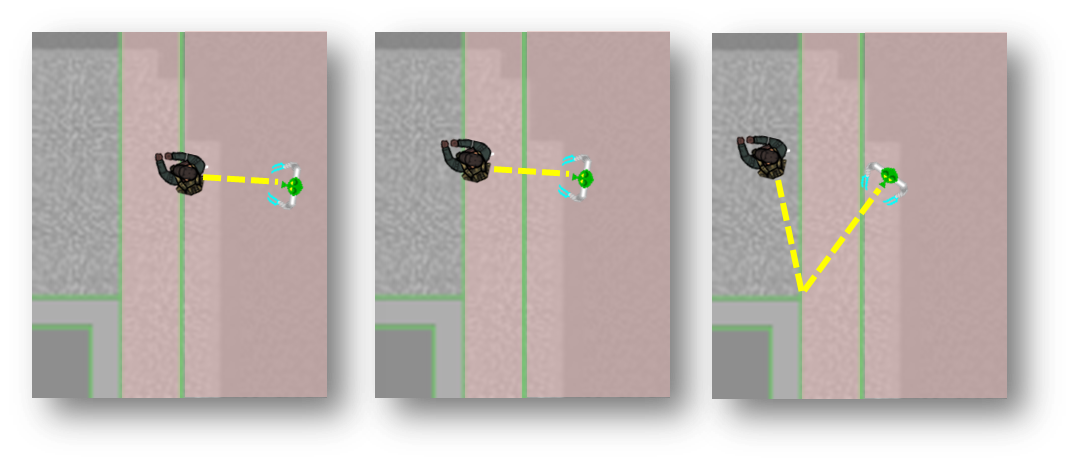
\includegraphics[width=\textwidth]{figures/astar/tradeoff.png}
    \caption{Illustration of the problem with small partitions with low waypoint count. Red partitions shows the partitions of the enemy.}\label{tradeoff}
\end{center}
\end{figure}
